\chapter{Capitolo 3: Albero Evolutivo}
Una delle sfide più importanti della bioinformatica, nonché l'obiettivo principale della filogenetica, è la costruzione degli alberi evolutivi.
\newline
Ricordando la definizione di albero, ovvero un grafo non orientato connesso e aciclico \cite{algoritmiEStruttureDati2}, \textit{L'albero evolutivo} o \textit{albero filogenetico} è un diagramma che rappresenta le relazioni evolutive tra i vari organismi (animali, piante, virus e così via) \cite{buildingaphylogenictree}. La sua peculiarità consiste nel poterli costruire utilizzando dati diversi tra loro, mostrando quindi relazioni di natura genetica, genomica o morfologica.
\newline
Gli alberi evolutivi possono essere suddivisi in due categorie: alberi radicati e non radicati.


\section{Albero radicato}
\begin{figure}[h!]
	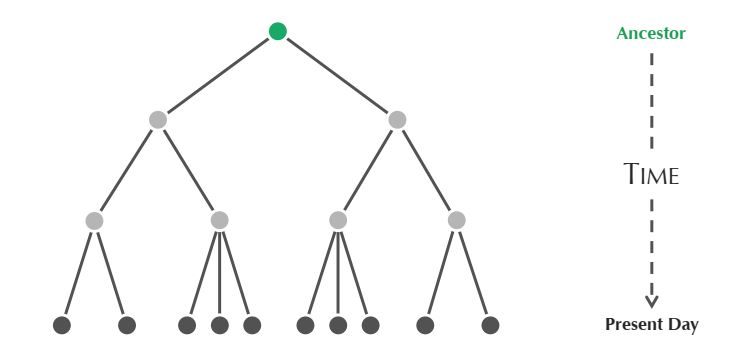
\includegraphics[width=\linewidth]{rooted_tree.jpg}
 	\caption{Un esempio di albero radicato.}
  	\label{fig:RootedTree}
\end{figure}
\textit{L'albero radicato} o \textit{albero con radice} è un albero in cui i nodi (o vertici) rappresentano gli organismi, mentre gli archi rappresentano la loro evoluzione nel tempo (figura 2) \cite{bioinfalganactivelearningapproachparttwo}. Esso si sviluppa a partire da un nodo speciale, chiamato \textit{radice} (il vertice verde nella figura) e si estende fino alle foglie. I vertici che hanno grado\footnote{Il grado di un vertice \textit{v} è dato dal numero degli archi incidenti su \textit{v} \cite{algoritmiEStruttureDati2}.} maggiore di uno, definiti \textit{nodi interni}, sono gli antenati, mentre quelli con grado esattamente uguale ad uno, definite \textit{foglie}, sono le forme di vita attualmente esistenti. La radice, quindi, è l'antenato comune a tutti i vertici dell'albero.
\newline
Il suo utilizzo non si riconduce solo alla conoscenza della radice, ma anche ai legami tra gli organismi.
\newline
\begin{figure}[h!]
	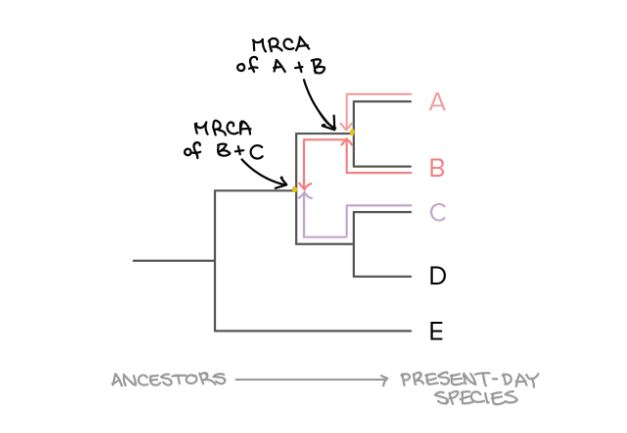
\includegraphics[width=\linewidth]{rooted_tree_2.jpg}
 	\caption{Un esempio di albero radicato che mostra le relazioni tra gli organismi.}
  	\label{fig:RootedTree}
\end{figure}
\newline
Come mostrato nella figura 3, gli organismi risultano più legati tra loro rispetto agli altri se hanno l'antenato più recente in comune, ad esempio A è più legato a B piuttosto che a C. La sigla "MRCA", infatti, indica il Most Recent Common Ancestor.
\newline
Nel caso in cui non è presente la radice, si parla di albero non radicato.


\section{Albero non radicato}
\begin{figure}[h!]
	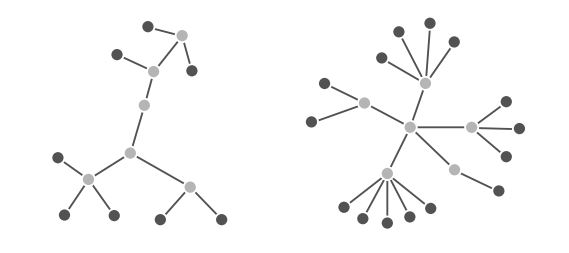
\includegraphics[width=\linewidth]{unrooted_trees.jpg}
 	\caption{Esempi di alberi non radicati.}
  	\label{fig:RootedTree}
\end{figure}
\textit{L'albero non radicato} o \textit{albero senza radice} è un albero in cui i nodi rappresentano gli organismi, mentre gli archi rappresentano la loro relazione, pertanto non richiedono la conoscenza della radice (figura 4) \cite{bioinfalganactivelearningapproachparttwo}.
\newline
Una domanda che può sorgere spontanea è perché usare gli alberi non radicati invece di quelli con radice. Le motivazioni sono molteplici.
\begin{itemize}
	\item Gli alberi senza radice possono essere considerati una generalizzazione di quelli radicati. Questo consente agli scienziati di formulare ipotesi più facilmente in merito alle relazioni tra organismi.
	\item Molti degli algoritmi utilizzati costruiscono alberi non radicati e solo successivamente viene trovata la radice, se necessario. Pertanto, rappresentano una parte importante della loro costruzione.
\end{itemize}


\section{Metodi per la costruzione degli alberi evolutivi}
Gli algoritmi utilizzati per la costruzione degli alberi evolutivi possono essere categorizzati in due metodologie:
\begin{itemize}
	\item \textit{Metodi basati sulla distanza}: vengono raccolti i dati in una matrice, definita matrice delle distanze, che viene usata per la costruzione degli alberi. Nel capitolo successivo ne verranno mostrati gli algoritmi;
	\item \textit{Metodi basati sui caratteri}: vengono usate le sequenze del DNA e delle proteine per la costruzione degli alberi.
\end{itemize}